% vim:set et sw=2 ts=4 tw=72:
\chapter{Design and Implementation}\label{cha:design_and_implementation}

In order to assess the usefulness of the model, it is necessary to
construct a tool that can be used for testing purposes. I designed and
built a tool called \tool{} to inspect and navigate through the
merge-trees representing the integrations into the kernel repository.
\tool{} is web-based to enable ease of use, requiring nothing more than
a web-browser to access, otherwise users would need to install the
software and the database of repository data.

\tool{} is designed with two uses-cases in mind, though a user may
freely switch between the cases as they work. Both use-cases are
designed with maintainers in mind.

\begin{textbox}
  \textbf{Use-Case 1: top-to-bottom approach}

  These users are maintaining a portion of the kernel and would like to
  pick and entire merge, including all commits being merged, and merge
  it directly into their version of the kernel.

  These users do not have a specific commit in mind.
\end{textbox}

\begin{textbox}
  \textbf{Use-Case 2: bottom-to-top approach}

  These are maintainers that start with a given commit and would like to
  understand what other changes are being made to integrate this commit.
  This is done by understanding the merges that the commit passes
  through toward integration, and finding the commits that are necessary
  for the integration of a given commit.

  These users do have a specific commit in mind.
\end{textbox}

While we designed \tool{} with Use-Case 1 in mind, Use-Case 2 is more
pertinent to our primary research questions. The tool uses full-text
search to gather the repository events that the user is interested in,
two summarization views, and three visualizations of the merge-tree for
the repository events.

\section{Search}\label{sec:search}

\evan{Should I put this section in the implementation details?}

\tool{} provides a search engine for navigating within the kernel
repository, filtering the repository events that are not relevant. The
search engine takes a plain-text query from the user and returns the
results ordered by the relevancy to the query. Relevancy is computed by
weighted similarity, taking into account the contents of the commit log,
the author name, the filenames, the commit hash, the date the commit was
authored, and the date the commit was committed.

Before presenting the results, the repository events are grouped by
merge-tree root. Each group of events has the link to the root at the
top, followed by a table of the relevant commits and merges from that
tree, shown in Figure~\ref{fig:linvis_search_results}. The table of
results includes the relevancy rank assigned by the search engine,
commit preview, author, commit date, and the authored date. The
merge-tree groups are ordered by the mean of the relevancy scores.

\begin{figure}[htpb]
  \centering
  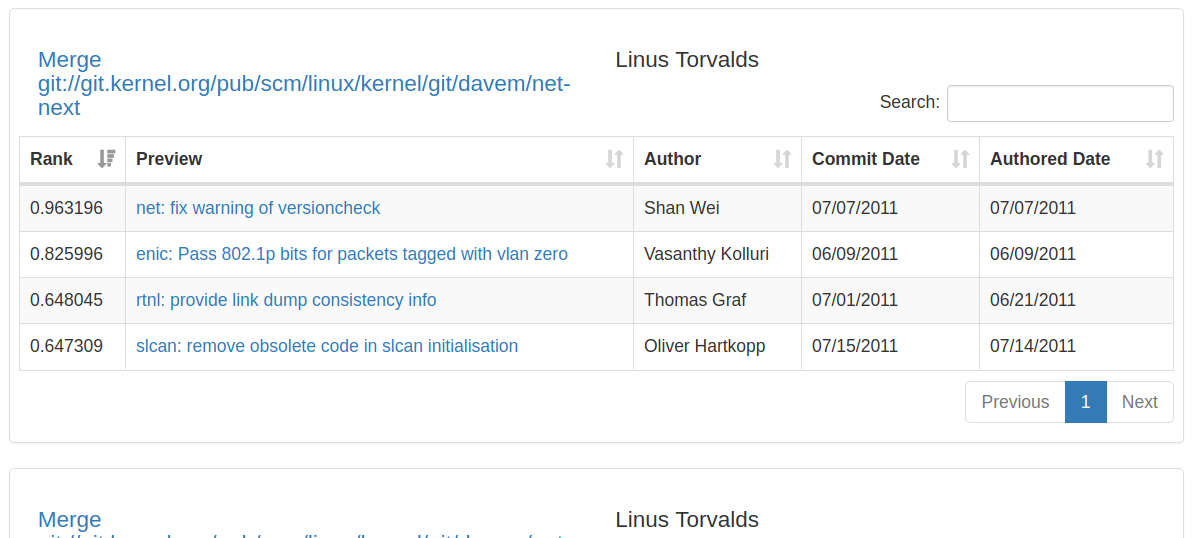
\includegraphics[width=0.8\linewidth]{Figures/Linvis/search_results.png}
  \caption{A single merge-tree in the search results of \tool{}, showing
    the link to the root at the top, and the relevant commits in the
    table below.}
  \label{fig:linvis_search_results}
\end{figure}
